\documentclass[12pt,a4paper]{article}

\usepackage[utf8]{inputenc}
\usepackage{graphicx}
\usepackage[spanish]{babel}
\usepackage{float}				%Para poner las imagenes exactamente donde se me cante las pelotas en caso de quererlo, poniendole [H]
\usepackage{amsmath}
\usepackage{epstopdf}
\usepackage{geometry}
\usepackage{hieroglf}
\usepackage{subcaption}
\usepackage[justification=centering]{caption}
\usepackage[colorinlistoftodos]{todonotes}
\usepackage[colorlinks=true, allcolors=blue]{hyperref}
\geometry{
a4paper,
left=20mm,
right=20mm,
top=25mm,
bottom = 20mm
}
\usepackage{float}
\usepackage{units}
% \usepackage{hyperref}   %Esto es para ir a los links

\newcommand{\rojo}[1]{\textcolor{red}{#1}}    % Comando para escribir texto en rojo




\title{\textbf{Redes Neuronales \\ Práctica 6 - Memorias asociativas}}

\author{
{F. M. Cabrera}
%[1ex] \small{\textit{ Facultad de Ciencias Exactas y Naturales.}} \\
%\small{\textit{Universidad de Buenos Aires. Ciudad Universitaria. Pabellón I. Buenos Aires. Argentina}}
}
\date{\textit{\today}}


% Esto modifica el interlineado
\renewcommand{\baselinestretch}{1}

\graphicspath{{../Figuras/}}

\begin{document}

\maketitle

%\thispagestyle{empty} 


\setcounter{page}{1}

%\begin{abstract}


%\end{abstract}
%\vspace*{1cm}

%  \rojo{Sacar esto \cite{HH}}


\section*{Ejercicio 1}
\graphicspath{{Figuras/}}

Para este ejercicio se busco resolver el problema de XOR a partir de dos arquitecturas distintas, las cuales pueden observarse en la Figura \ref{fig:1_Arquitecturas} y cuya principal diferencia es que una presenta una reinyección de la entrada mientras que otra no. En ambos casos, la función de activación de la capa oculta fue $\tanh$ y como función de costo se utilizo MSE. Debido a que la función de activación utilizada nunca retorna $1$ o $-1$, se determino un umbral de 0.9 en la función de costo, de manera que si el resultado supera dicho umbral, se considera la salida como 1. De manera análoga, se determino un segundo umbral de -0.9 para determinar cuando la salida se considera un -1.

\begin{figure}[h!]
    \centering
    \begin{subfigure}[h]{0.3\textwidth} 
        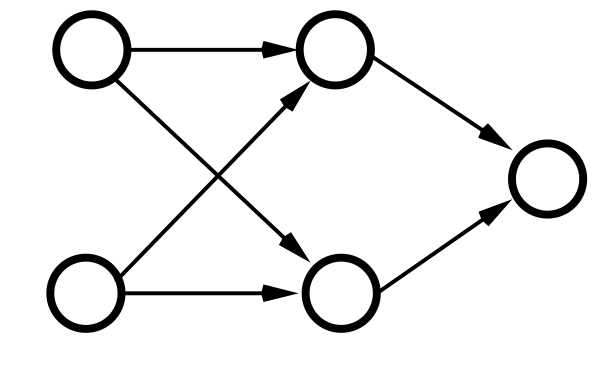
\includegraphics[width=\textwidth]{Figuras/ejer_1_221.png}
    \end{subfigure}       
    \begin{subfigure}[h]{0.3\textwidth} 
        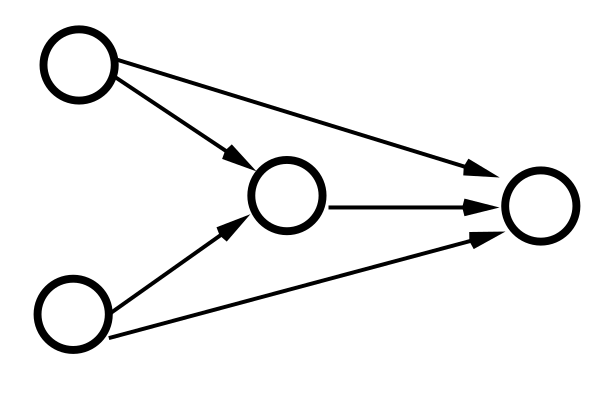
\includegraphics[width=\textwidth]{Figuras/ejer_1_211.png}
    \end{subfigure}
    \caption{Esquema de las arquitecturas utilizadas para resolver el problema del XOR.} \label{fig:1_Arquitecturas}
\end{figure}

En ambos casos se utilizo la totalidad de los datos como datos de entrenamiento. Los resultados para la función de costo y el \textit{accuracy} para la primer arquitectura en 10 procesos de entrenamiento independientes de la red pueden observarse en la Fig. \ref{fig:1_1erArquitectura}, mientras que en la Fig. \ref{fig:1_2daArquitectura} se observan los resultados análogos para la segunda arquitectura. En ambos casos se observa que algunos procesos de entrenamiento no convergen y no alcanzan un valor de \textit{accuracy} optimo del $100\%$.

\begin{figure}[h!]
    \centering
    \begin{subfigure}[h]{0.49\textwidth} 
        \includegraphics[width=\textwidth]{Figuras/ej1_1erArquitectura/Acc.pdf}
    \end{subfigure}       
    \begin{subfigure}[h]{0.49\textwidth} 
        \includegraphics[width=\textwidth]{Figuras/ej1_1erArquitectura/Loss.pdf}
    \end{subfigure}
    \caption{Función de costo MSE y \textit{accuracy} para el entrenamiento de 10 modelos independientes, utilizando la primer arquitectura propuesta en Fig. \ref{fig:1_Arquitecturas}.} \label{fig:1_1erArquitectura}
\end{figure}

\begin{figure}[h!]
    \centering
    \begin{subfigure}[h]{0.49\textwidth} 
        \includegraphics[width=\textwidth]{Figuras/ej1_2daArquitectura/Acc.pdf}
    \end{subfigure}       
    \begin{subfigure}[h]{0.49\textwidth} 
        \includegraphics[width=\textwidth]{Figuras/ej1_2daArquitectura/Loss.pdf}
    \end{subfigure}
    \caption{Función de costo MSE y \textit{accuracy} para el entrenamiento de 10 modelos independientes, utilizando la segunda arquitectura propuesta en Fig. \ref{fig:1_Arquitecturas}.} \label{fig:1_2daArquitectura}
\end{figure}

Se definió el tiempo de convergencia como aquella época en donde la función de costo alcanza un valor de $0.1$, pero solo para los modelos que convergieron a una solución optima dentro de las $2000$ épocas. Para comparar los tiempos de convergencia entre ambas arquitecturas, se entrenaron 1000 modelos independientes que lograron converger y se obtuvo su tiempo de convergencia, para ambas arquitecturas. Para la primer arquitectura se obtuvo un tiempo de convergencia promedio de $157.5$ épocas, mientras que para la segunda se obtuvo un valor de $148.7$. En principio, esta diferencia, aunque sea pequeña, podría indicar que la segunda arquitectura es mejor para la resolución del problema XOR. Sin embargo, para obtener 1000 modelos entrenados que hayan logrado converger a una solución optima, fue necesario entrenar 1288 modelos para la primer arquitectura, mientras que para la segunda fueron necesarios 1983. Es decir, que el $77.6\%$ de los modelos creados con la primer arquitectura lograron converger, mientras que para la segunda solo el $50.4\%$, lo cual apunta a que la primer arquitectura es mas satisfactoria para resolver el problema.
\section*{Ejercicio 2}
\graphicspath{{Figuras/}}

Se busco estudiar una generalización del problemas de XOR para $N$ entradas, en donde la salida esperada es el producto de todas las componentes de la entrada. La arquitectura utilizada consistió en una capa oculta de $N'$ neuronas con una función de activación \texttt{tanh}, seguida de una capa de salida de 1 neurona tambien con activacion \texttt{tanh}. Debido a que la cantidad de datos de entrada es igual a $2^{N}$ y era de interés estudiar los casos en donde $N>N'$ y $N<N'$, se fijo $N$ a un valor de 5 y se entreno la red para distintos valores de $N'$: 1, 3, 5, 7, 9 y 11, en todos ellos durante 5000 épocas.

\begin{figure}[h!]
    \centering
    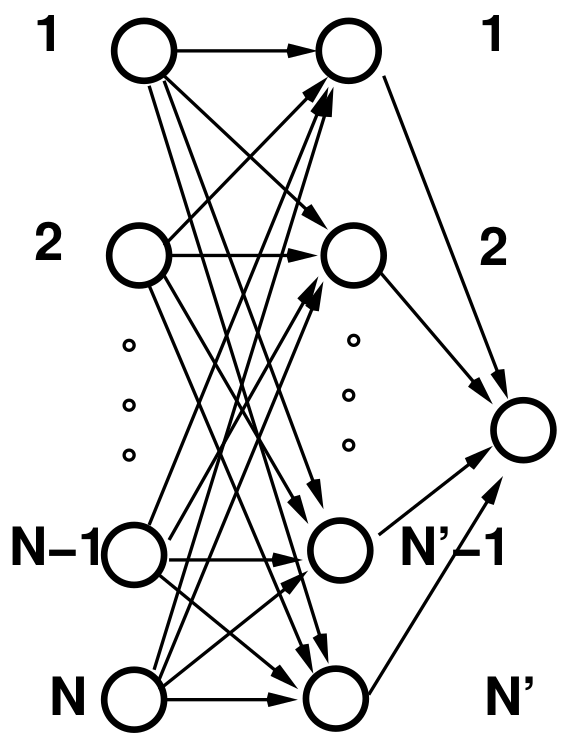
\includegraphics[width=0.3\textwidth]{Figuras/ejer_2_NN1.png}
    \caption{Esquema de la arquitectura utilizada para resolver el problema del XOR generalizado.}
    \label{02:fig:Arquitectura}
\end{figure}

En la Figura \ref{fig:2_Resultados} se observan los resultados obtenidos para la función de costo y \textit{accuracy} en cada uno de los casos. En caso de que $N'>N$, los resultados son similares a los del ejercicio anterior, ya que en una pequeña cantidad de épocas se obtiene un 100\% de precisión. La situación se vuelve mas problemática al disminuir $N'$, en donde se observa que para $N'=N=5$ el aprendizaje de la red nunca alcanza una precisión total e incluso no mejora de manera monótona conforme avanzan las épocas. Los resultados son incluso peores cuando $N'<N$, en donde se requieren muchas mas épocas para que la red aprenda e incluso para $N'=1$ nunca se logra alcanzar un valor de \textit{accuracy} no nulo. Este problema es esperable, ya que el valor de $N'$ determina las dimensiones de las matrices de pesos de cada una de las capas. Al disminuir $N'$, menor sera la cantidad de componentes de estas matrices, con lo cual deberá ajustar una gran cantidad de datos de entrada ($2^{N}$) con menos grados de libertad, que, en caso de ser demasiado pocos, se presentara un problema de underfitting y la red no mejorara sus resultados.


\begin{figure}[h!]
    \centering
    \begin{subfigure}[h]{0.49\textwidth} 
        \includegraphics[width=\textwidth]{Figuras/ej2/Acc.pdf}
    \end{subfigure}       
    \begin{subfigure}[h]{0.49\textwidth} 
        \includegraphics[width=\textwidth]{Figuras/ej2/Loss.pdf}
    \end{subfigure}
    \caption{Función de costo MSE y \textit{accuracy} para el entrenamiento de 6 modelos independientes variando la cantidad de neuronas de la capa oculta, utilizando la arquitectura propuesta en Fig. \ref{fig:1_Arquitecturas}.}
    \label{fig:2_Resultados}
\end{figure}



% \bibliographystyle{acm}
% \bibliography{biblio}

\end{document}



